\begin{center}
  {\LARGE\bfseries Prof. Debasish Ghose Maps the Future of AI, Autonomy and Swarming at STCET\par}
  \vspace{0.45em}
  {\large\bfseries\color{IEEEblue}
  IISc aerospace expert links multi-robot intelligence with defence, deep-space navigation and the next generation of scientific missions.\par}
  \vspace{0.5em}
  {\small\itshape By the Editorial Desk}
\end{center}

\begin{tcolorbox}[
  colback=SoftBlue,
  colframe=IEEEblue!75!black,
  boxrule=0.6pt,
  arc=0mm,
  left=3mm,right=3mm,top=2mm,bottom=2mm
]
  \small\RaggedRight
  \textbf{At a glance:} Prof. Debasish Ghose of the Department of Aerospace Engineering, Indian Institute of Science (IISc), Bengaluru, delivered the technical talk ``Towards Innovation on AI, Autonomy and Swarming'' at noon on February 16, 2026, in the STCET Seminar Hall. The programme was organised by the IEEE Student Branch--STCET with the IEEE CIS \& IES Student Chapter, IEEE WIE Student Branch Affinity Group, Institution's Innovation Council (IIC), and Research \& Development Cell, STCET.
\end{tcolorbox}

\begin{center}
  \setlength{\tabcolsep}{2pt}
  \begin{tabular}{@{}cc@{}}
    \includegraphics[height=0.4\textheight]{assets/images/aas-2.jpeg} &
    \includegraphics[height=0.4\textheight]{assets/images/aas3.jpeg}
  \end{tabular}

  \vspace{2pt}
  {\footnotesize\itshape Speakers introduce the technical session on AI, autonomy and swarming.\par}
\end{center}

{\small
\noindent
\textbf{Kolkata, February 16, 2026---}Artificial intelligence moved from the screen into the physical world during a distinguished technical talk at St. Thomas' College of Engineering \& Technology (STCET), where Prof. Debasish Ghose of IISc Bengaluru examined how autonomous machines can navigate, cooperate and make decisions as a group. The session on ``Towards Innovation on AI, Autonomy and Swarming'' was jointly supported by the IEEE CIS \& IES Student Chapter, the IEEE WIE Student Branch Affinity Group, the Institution's Innovation Council (IIC), and the Research \& Development Cell, STCET, under the IEEE Student Branch.

\medskip
\noindent
Prof. Ghose, whose research centres on the guidance and control of autonomous vehicles, introduced the audience to a field reshaping aerospace engineering, robotics and intelligent defence systems. His central message was that autonomy is more than automation. An automated machine follows a predetermined sequence; an autonomous system must sense its surroundings, interpret incomplete information, choose a course of action and adjust when conditions change.

\medskip
\noindent
That distinction becomes especially important when several robots or vehicles work together. A multi-robot system can divide a large task among many relatively simple agents, allowing the group to search a wider area, respond from multiple directions and continue operating even if one member fails. The engineering challenge is to coordinate the agents without creating excessive communication, computation or dependence on a single controller.

\medskip
\noindent
The lecture used swarm intelligence to explain how local decisions can produce useful collective behaviour. Natural swarms offer familiar examples: individual birds, insects or fish respond mainly to nearby neighbours, yet the group can move cohesively, avoid obstacles and adapt to threats. In engineered swarms, carefully designed algorithms translate similar principles into rules for alignment, separation, formation, task allocation, consensus and cooperative search.

\medskip
\noindent
Prof. Ghose highlighted that effective swarm behaviour does not emerge from imitation alone. Each agent requires sensing, localisation, communication and control, while the group needs algorithms that remain stable when information is delayed, noisy or incomplete. Designers must decide how much intelligence belongs on each vehicle, what information should be shared, and how the system should respond when communication links disappear or an agent behaves unexpectedly.

\begin{center}
  \setlength{\tabcolsep}{2pt}
  \begin{tabular}{@{}cc@{}}
    \includegraphics[height=0.4\textheight]{assets/images/aas-4.jpeg} &
    \includegraphics[height=0.4\textheight]{assets/images/aas-5.jpeg}
  \end{tabular}

  \vspace{2pt}
  {\footnotesize\itshape Moments from the lecture and the felicitation of the invited speaker.\par}
\end{center}

\medskip
\noindent
Dynamic path planning formed another major strand of the discussion. Unlike route planning on a fixed map, autonomous navigation often takes place in environments that change while a mission is under way. Obstacles may move, weather may deteriorate, targets may shift and new information may arrive from other agents. A practical planner must continually update a route while respecting constraints such as energy, turning radius, collision risk, sensor range and mission priority.

\medskip
\noindent
For a single vehicle, these requirements are already demanding. For a swarm, path planning becomes a coupled problem: every agent must make progress toward the mission objective without colliding with teammates or duplicating work unnecessarily. Distributed algorithms can allow vehicles to negotiate roles, maintain formations, exchange local observations and reassign tasks when circumstances change. The result is a system whose capability comes from coordination rather than from one exceptionally powerful machine.

\medskip
\noindent
The aerospace and defence relevance of these ideas was evident throughout the talk. Groups of unmanned aerial vehicles can support wide-area surveillance, disaster assessment, mapping, search operations and inspection of hazardous regions. Cooperative systems can cover terrain faster than a single platform, observe an object from several viewpoints and maintain a mission despite individual failures. Similar principles can guide marine robots, ground vehicles and mixed teams operating across air, land and water.

\medskip
\noindent
Prof. Ghose also connected autonomous swarms with the challenges of space exploration and astronomical observation. Satellite constellations increasingly depend on coordinated scheduling, relative positioning and communication across many spacecraft. Instead of treating each satellite as an isolated platform, autonomy can help a constellation distribute observations, manage resources and respond to changing mission priorities with less continuous intervention from the ground.

\medskip
\noindent
Deep-space missions create an even stronger case for onboard intelligence. Communication delays make immediate human control impossible when a spacecraft or planetary robot is far from Earth. Autonomous navigation must combine sensor data, estimate position, detect hazards and select safe actions locally. A group of small robotic explorers could potentially survey a larger planetary region, share discoveries and redirect one another toward scientifically important targets.

\begin{center}
  \setlength{\tabcolsep}{2pt}
  \begin{tabular}{@{}cc@{}}
    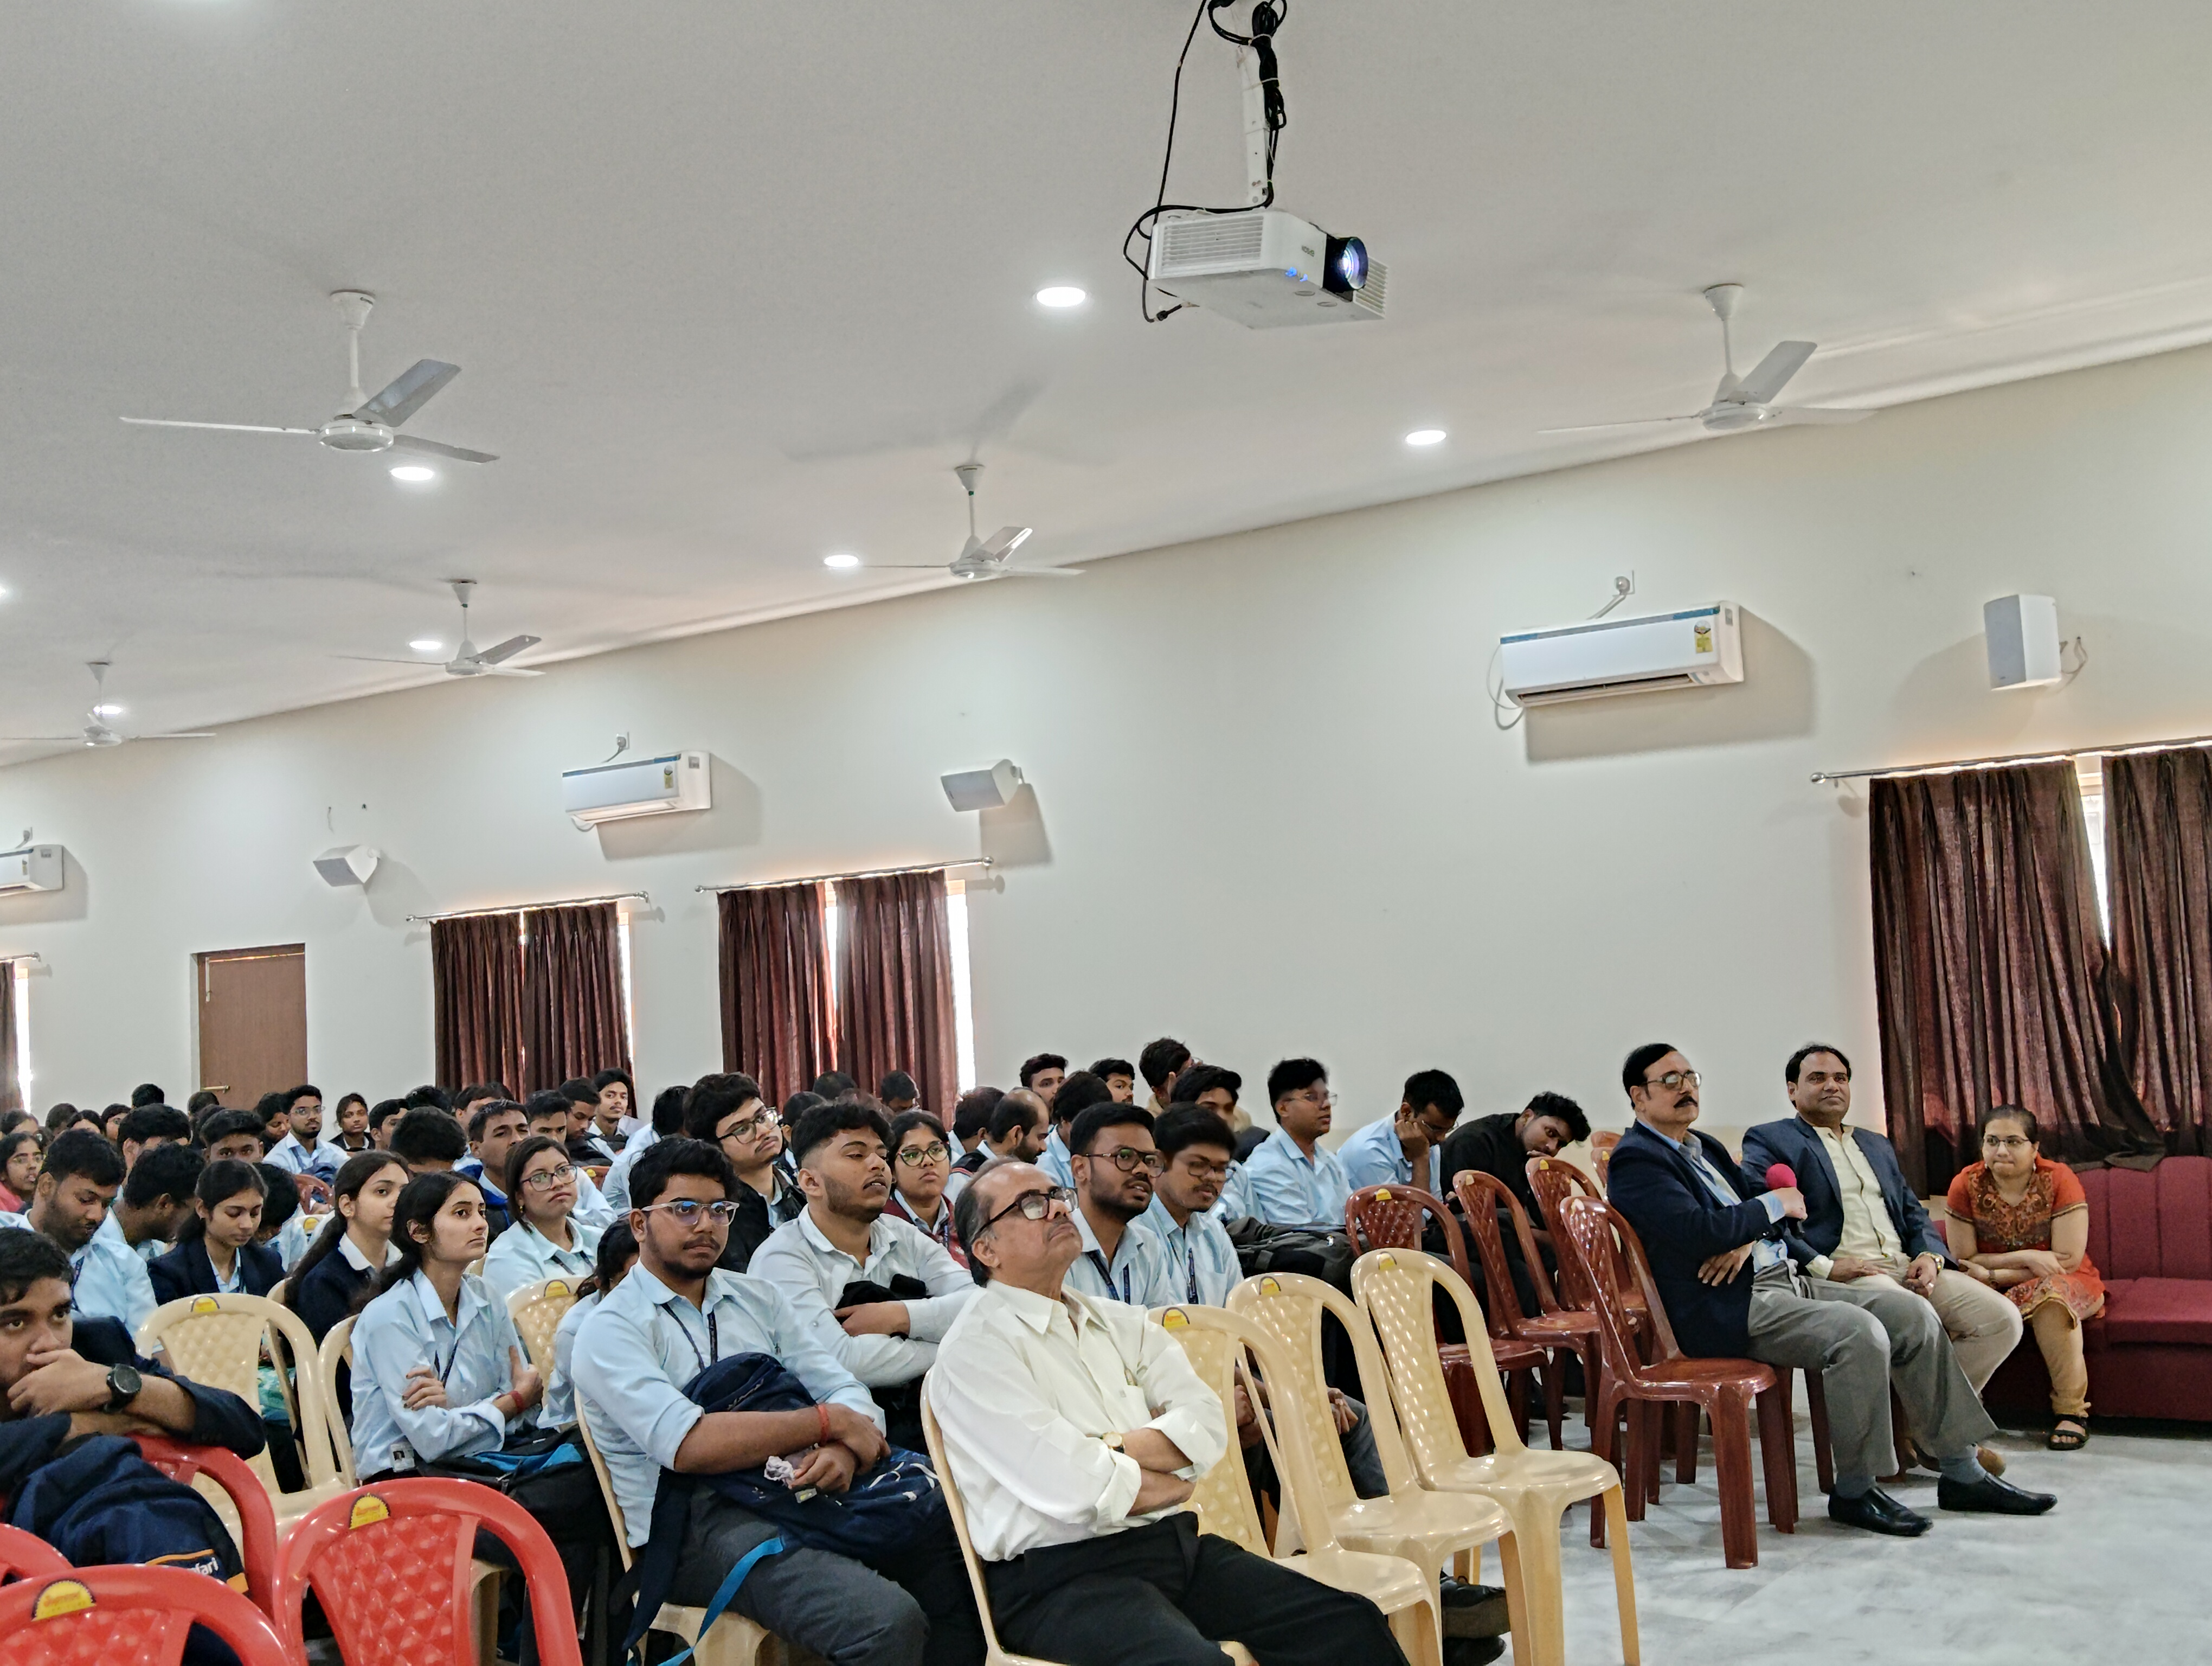
\includegraphics[width=0.45\textwidth]{assets/images/aas-6.jpeg} &
    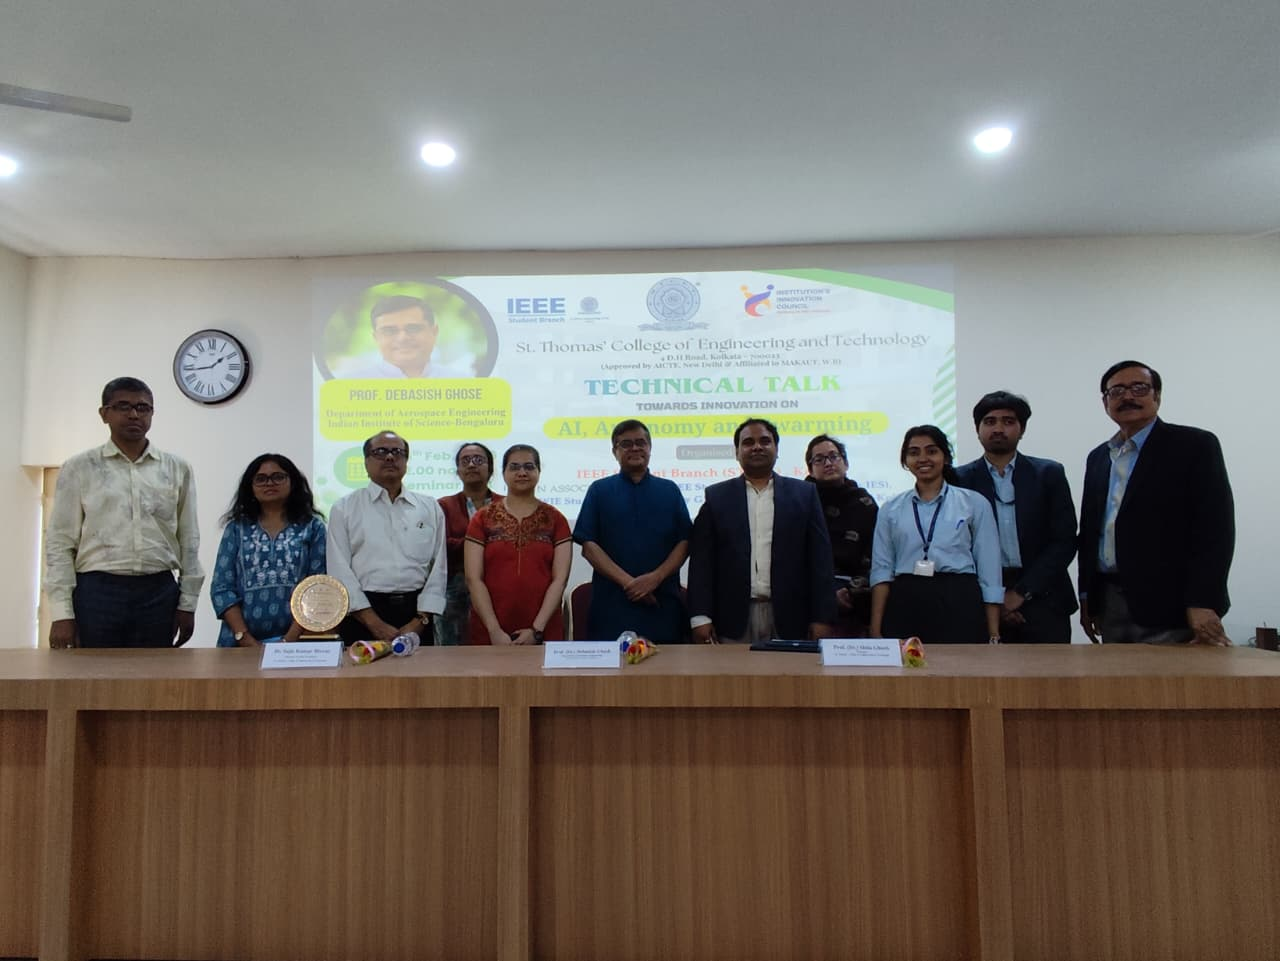
\includegraphics[width=0.45\textwidth]{assets/images/aas-7.jpeg}
  \end{tabular}

  \vspace{2pt}
  {\footnotesize\itshape The attentive audience and organisers at the conclusion of the programme.\par}
\end{center}

\medskip
\noindent
In astronomical missions, coordinated spacecraft can observe the same phenomenon from different locations or divide a survey among several instruments. Swarming concepts could support distributed sensing, formation flying and interferometric observations in which measurements from separated platforms are combined. Such missions demand extraordinary precision: small navigation or timing errors can degrade the scientific result, making guidance, synchronisation and fault-tolerant control as important as the telescope or detector itself.

\medskip
\noindent
The lecture balanced this technological promise with the limits that engineers must confront. Autonomous systems can fail because of poor training data, sensor errors, unforeseen conditions, cyberattack or an objective function that does not reflect the real mission. In defence and other safety-critical applications, decisions may also carry ethical and legal consequences. Human oversight, explainability, secure communication, testing and clearly defined authority therefore remain essential even as machines gain greater independence.

\medskip
\noindent
These concerns carried into the interactive question-and-answer session. Students, IEEE members and faculty participants engaged Prof. Ghose on the trustworthiness of AI decisions, the balance between centralised and distributed control, and the difficulty of guaranteeing safe collective behaviour. Questions also explored how engineers can prevent a swarm from amplifying one faulty decision across the entire group.

\medskip
\noindent
Young researchers sought guidance on entering the field, prompting discussion of the foundations required for meaningful work in autonomy: mathematics, control theory, optimisation, programming, robotics, probability, signal processing and machine learning. The exchange made clear that autonomous-systems research is inherently interdisciplinary. Progress depends on researchers who can connect algorithms with sensors, actuators, communication limits and the physical dynamics of real vehicles.

\medskip
\noindent
The programme's joint organisation reflected this breadth. The IEEE CIS community contributed the perspective of computational intelligence; the IES chapter connected intelligent algorithms with electronics and industrial systems; IEEE WIE reinforced inclusive participation in advanced technology; and the IIC and R\&D Cell placed the discussion within STCET's wider culture of innovation and research.

\medskip
\noindent
For students, the talk offered more than a survey of an emerging field. It showed how concepts learned separately in classrooms---feedback control, embedded systems, communication networks, optimisation and AI---come together in machines that must act reliably in the real world. It also demonstrated why research problems at the frontier rarely belong to one department or one branch of engineering.

\medskip
\noindent
By the close of the session, autonomy had been presented neither as effortless machine intelligence nor as a distant futuristic idea. It emerged as a demanding engineering discipline built on models, evidence, careful testing and responsible design. Prof. Ghose's talk left the audience with a compelling picture of the future: fleets of machines capable of cooperating across Earth and space, provided that human ingenuity is matched by technical rigour and ethical judgement.
\par}

\begin{center}
  \includegraphics[width=\textwidth]{assets/images/aas-1.jpeg}

  \vspace{2pt}
  {\footnotesize\itshape The technical talk in progress at the STCET Seminar Hall.\par}
\end{center}

\vfill
\noindent
{\footnotesize\sloppy\textit{Source note: Event title, date, time, venue and organising details are based on the official STCET event listing and programme announcement. Professional details are based on the official IISc Aerospace Engineering profile of Prof. Debasish Ghose.}\par}